\chapter{Conceitos Centrais em Estatística Inferencial}

Neste capítulo você vai rever os conceitos fundamentais em estatística inferencial, que vão habilitá-lo a realizar teste de hipóteses estatisticamente significativas.
O capítulo é complementado por slides.

\section{Introdução}

Assista aos cinco vídeos a seguir indicados, que apresentarão a você vários conceitos necessários para que você aprende os conceitos fundamentais do teste de hipóteses, que serão úteis à conclusão do seu laboratório.

\begin{description}
\item [Inferência (\url{https://www.youtube.com/watch?v=FM9tz8U2g2k})] Esse vídeo aborda os dois tipos fundamentais de problemas que a inferência resolve:
\begin{enumerate}
    \item Estimar parâmetros para uma população (média, desvio padrão etc);
    \item Provar ou verificar hipóteses acerca das diferenças existentes entre duas ou mais populações, baseado na coleta de amostras.
\end{enumerate}
Em função a abordagem experimental, estamos mais interessados no segundo tipo de problema.

Ao assistir ao vídeo você deve procurar compreender o que significam cada um dos principais conceitos abordados, que são: 
\begin{enumerate}
    \item Inferência;
    \item Hipótese nula ($H_0$) e hipótese complementar ou hipótese alternativa ($H_1$);
    \item Amostragem aleatória;
    \item Distribuição normal;
    \item Intervalo ou nível de confiança; 
    \item Amostragens de grupos independentes; 
    \item Seleção de teste estatístico (student, chi-quadrado, ANOVA);
    \item critério de teste;
    \item Região de rejeição e região(ões) de aceitação;
    \item Valor crítico de um teste;
    \item Tipos de erros em teste de hipótese (falso negativo - - Erro tipo I e falso positivo erro tipo II);
    \item Controle de tipos de erros;
    \item Teorema do Limite Central;
    \item Média, variância e desvio padrão.
\end{enumerate}

\item [Choosing a Statistical Test for Your IB Biology IA] O vídeo em \url{https://www.youtube.com/watch?v=ulk_JWckJ78} apresenta um sumário da aplicabilidade de vários testes estatísticos, sendo os principais:
\begin{enumerate}
    \item Chi-quadrado;
    \item Teste t, de student;
    \item Teste de regressão linear;
\end{enumerate}


\item [Teste Chi-Quadrado (\url{https://www.youtube.com/watch?v=4QfHVbpAoSg})] Apresenta como calcular e usar o Teste Chi-Quadrado, um teste não paramétrico que usa a medida frequência (em vez de média, por exemplo) para comparar diferentes amostras (independentes) em uma tabela de contingência. Por usar a frequência, o Chi-Quadrado é útil para verificar hipóteses quando a variável dependente é nominal, ordinal ou intervalar. 

Ao assistir o vídeo, procure compreender o significado dos principais conceitos abordados, que são:
\begin{enumerate}
    \item Amostragem aleatória;
    \item Distribuição normal;
    \item Teste Chi-Quadrado com um critério, e com dois grupos;
    \item Método não paramétrico;
    \item Tabelas de contingência (tabela cruzada, cross-table);
    \item Cálculo do valor do teste Chi-Quadrado para uma amostra;
    \item Graus de liberdade;
    \item Valor crítico do Chi-Quadrado;
    \item Significância do teste.
\end{enumerate}
Você deve procurar compreender o que significam cada um desses conceitos.
\item [Teste t (de Student) (\url{https://www.youtube.com/watch?v=AgDC9yoopUA})] apresenta como calcular o teste T para amostras independentes, método baseado no parâmetro média, que permite comparar as diferenças das médias de diferentes pares de amostras.
Principais conceitos abordados no vídeo:
\begin{enumerate}
    \item Amostragem aleatória;
    \item Distribuição normal;
    \item Teste t, que permite comparar dois grupos;
    \item Método paramétrico (usa o parâmetro média);
    \item Cálculo do valor do teste t para uma amostra;
    \item Graus de liberdade;
    \item Valor crítico do teste t;
    \item Significância do teste t.
\end{enumerate}

\item [ANOVA - Análise de variância (\url{https://www.youtube.com/watch?v=1ceP2FL5fzE})] Apresenta o teste ANOVA, usado para comparar médias entre três ou mais grupos.
Principais conceitos abordados no vídeo:
\begin{enumerate}
    \item Amostragem aleatória;
    \item Distribuição normal;
    \item Teste de normalidade (Kolmogorov-Smirnov);
    \item variação intra e entre grupos;
    \item Cálculo do valor do teste ANOVA para uma amostra (F crítico);
    \item Graus de liberdade;
    \item Valor crítico do teste;
    \item Significância do teste.
\end{enumerate}
Você deve procurar compreender o que significam cada um desses conceitos.

\end{description}

\section{Slides}

Veja slides neste projeto Overleaf, em 
4-Computacao-Experimental/aulas/4.4-Teste-Hipoteses/slides-estatistica-inferencial.pdf

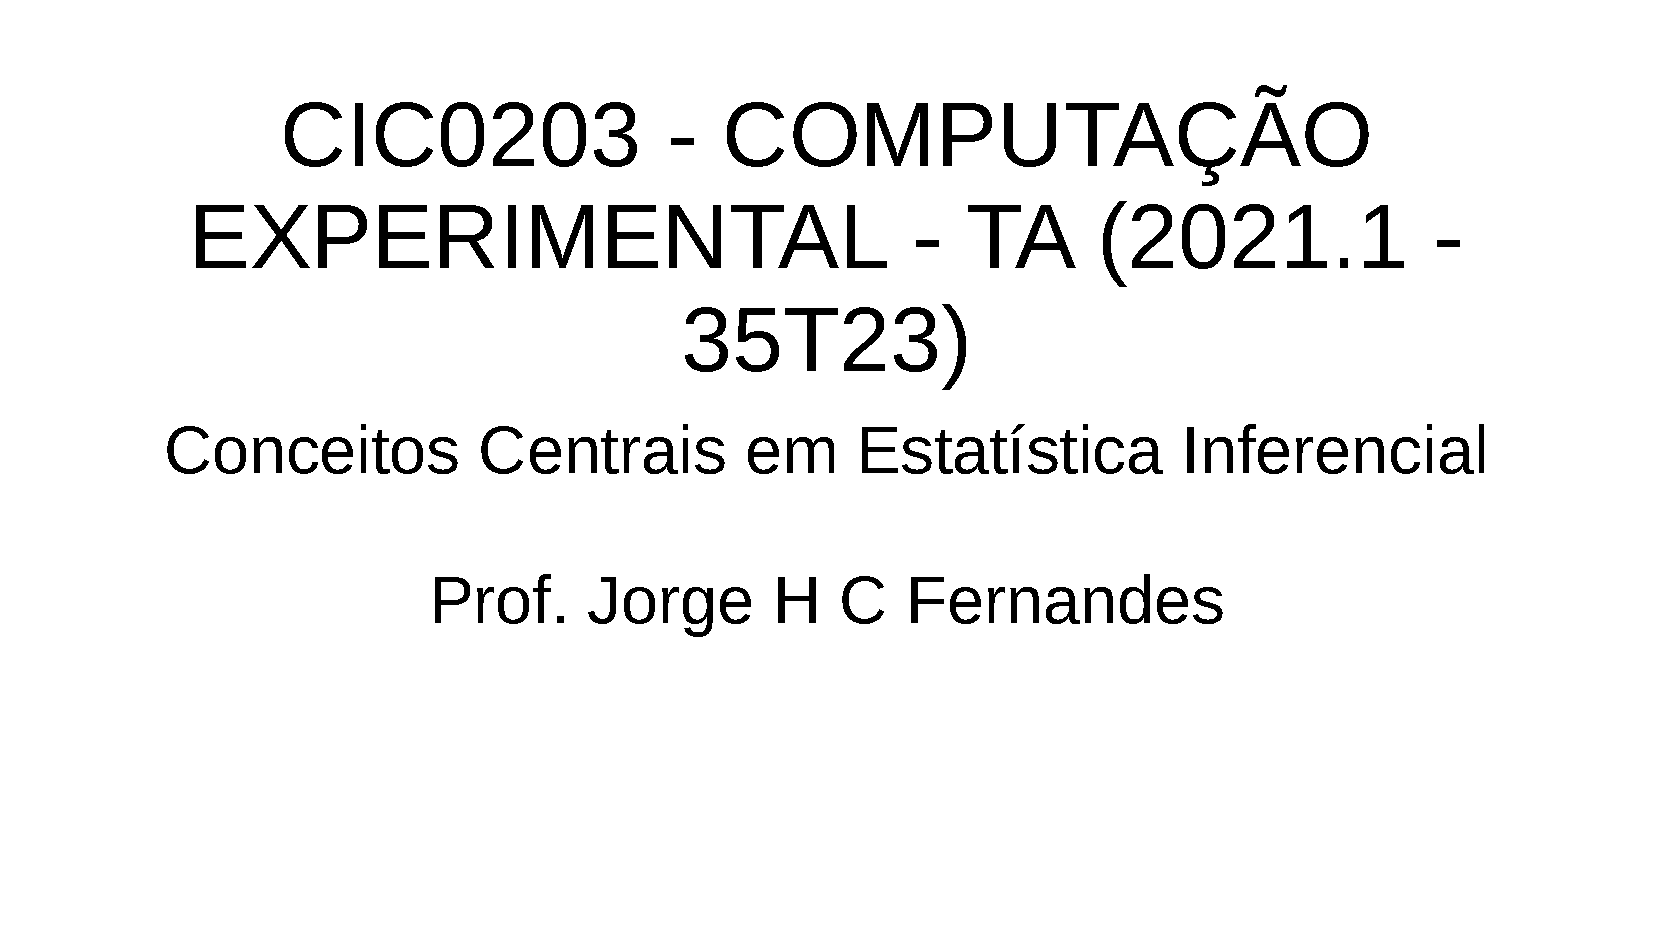
\includepdf[pages=-]{4-Computacao-Experimental/aulas/4.4-Teste-Hipoteses/slides-estatistica-inferencial.pdf}


Após estudar cuidadosamente os quatro vídeos faça a tarefa especificada a seguir

